\section{Câu 7}
Cho một tín hiệu cần xử lý dưới dạng dòng điện, có tầm thay đổi từ 1mA – 10mA.

a. Thiết kế mạch cho ngõ ra tầm 100mV – 1V.

b. Lựa chọn OPAMP và các linh kiện cần thiết để mạch hoạt động. Lưu ý: xử lý các
thông số không lý tưởng của OPAMP. (Tham khảo datasheet)    

\begin{center}
\textbf{Bài giải}
\end{center}

a. Để thiết kế mạch chuyển đổi tín hiệu dòng điện sang điện áp ta biểu diễn mối quan hệ giữa dòng điện và điện áp như hình bên dưới
\begin{figure}[H]
    \centering
    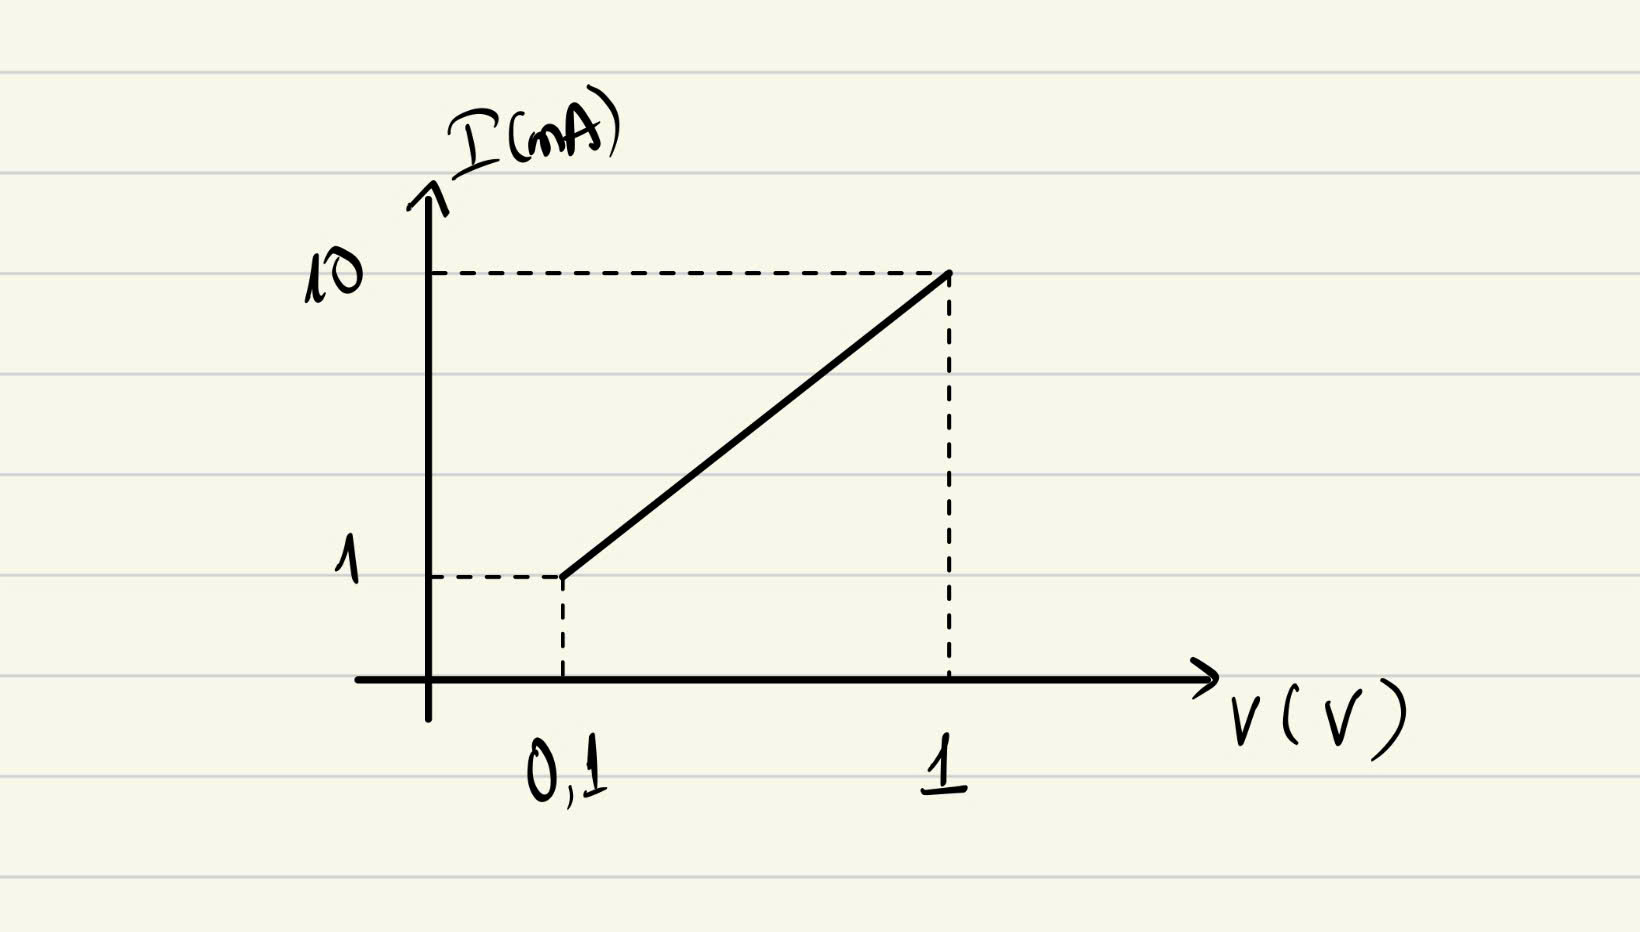
\includegraphics[scale=0.2]{image/C7_chart.jpg} 
\end{figure}
Từ hình trên ta có hệ phương trình:
\begin{equation*}
    \begin{cases}
        0.1 = 1\cdot a + b  \\
        1 = 10\cdot a + b\\
    \end{cases}
\end{equation*}
Giải hệ phương trình ta được:  
\begin{equation*}
    \begin{cases}
        a = 0.1\\
        b = 0 \\
    \end{cases}
\end{equation*}
Vậy ta có phương trình mạch chuyển đổi dòng điện sang điện áp như sau:
\begin{equation*}
    \boxed{V = 0.1I}
    \rightarrow \text{ Chọn } R = 100\Omega
\end{equation*}
\textbf{b.} Thiết kế mạch


Việc chọn giá trị điện được thực hiện như sau:
\begin{itemize}
    \item Các điện trở R$_3$ trong mạch khuếch đại chọn bằng 100\,$\Omega$ để làm giảm ảnh hưởng nhiễu.
    \item Giả sử tần số cắt f$_c$ = 10KHz, chọn tụ C như sau:
    \begin{equation*}
        C = \dfrac{1}{2\pi R f_c} = \dfrac{1}{2\pi \cdot 100\Omega \cdot 10KHz} = 159.15n F
    \end{equation*}
\end{itemize}

Chọn OPAMP OPA2333 vì các thông số tham khảo được:
\begin{itemize}
    \item Khả năng rail to rail ở ngõ ra: có.
    \item Vos (độ dịch chuyển ngõ vào): 2$\mu$V.
    \item Ib (dòng dịch chuyển ngõ vào): 2pA.
    \item Ios (dòng dịch chuyển bù ngõ vào): 140pA.
    \item Các sai số ngõ vào rất bé nhưng nguồn cấp khá nhỏ.
\end{itemize}
Mạch hoàn chỉnh như hình bên dưới:
\begin{figure}[H]
    \centering
    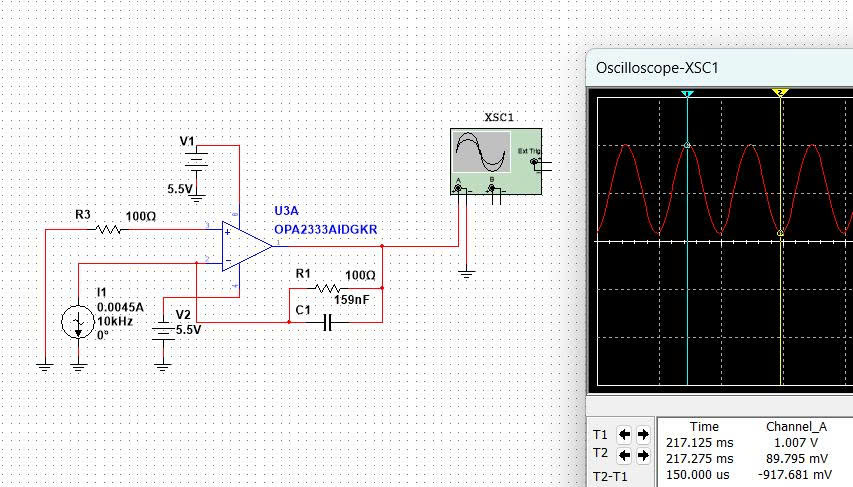
\includegraphics[scale=0.5]{image/C7.jpg}
\end{figure}